\chapter{Выполнение работы}

Для достижения поставленной цели необходимо:
\begin{enumerate}
	\item получить графовое представление заданного аудиофайла;
	\item преобразовать полученный граф путем смешивания с изображением пейзажем.
\end{enumerate}

\section{Графовое представление заданного аудиофайла}

На рисунке \ref{img:graph} изображено графовое представление заданного аудиофайла.
\begin{figure}[ht!]
	\centering
	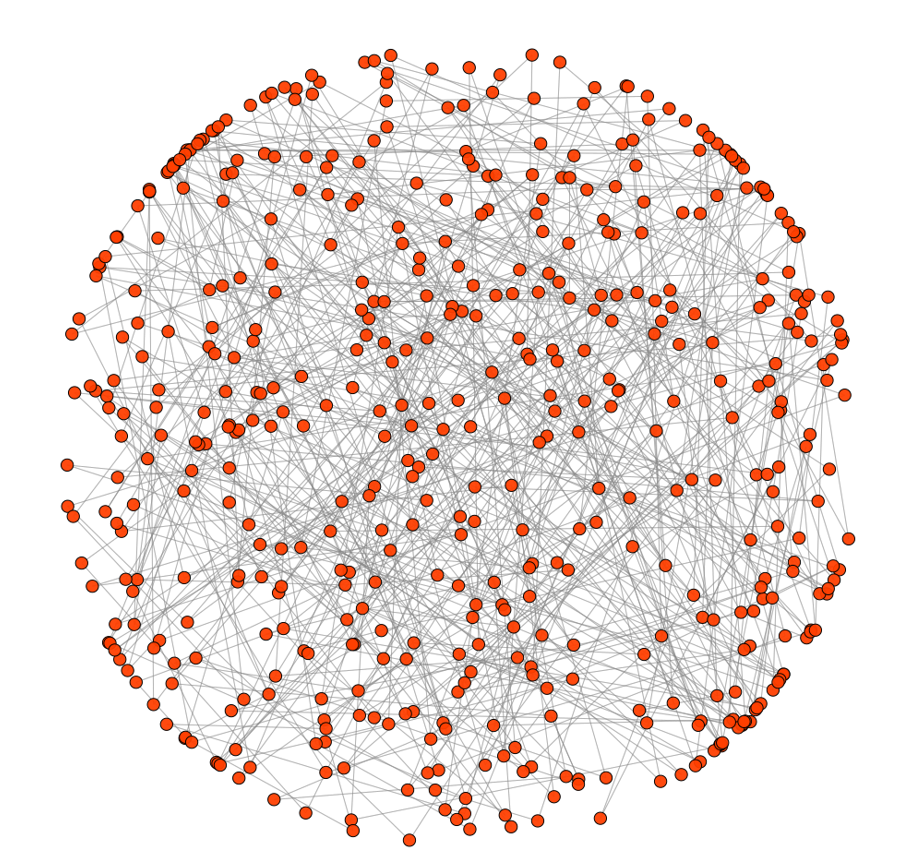
\includegraphics[width=170mm]{./img/graph1.png}
	\caption{Графовое представление заданного аудиофайла}
	\label{img:graph}
\end{figure}

\clearpage

\section{Преобразование полученного графа путем смешивания с изображением пейзажа}

На рисунке \ref{img:march} изображен исходный мартовский пейзаж для смешивания.
\begin{figure}[ht!]
	\centering
	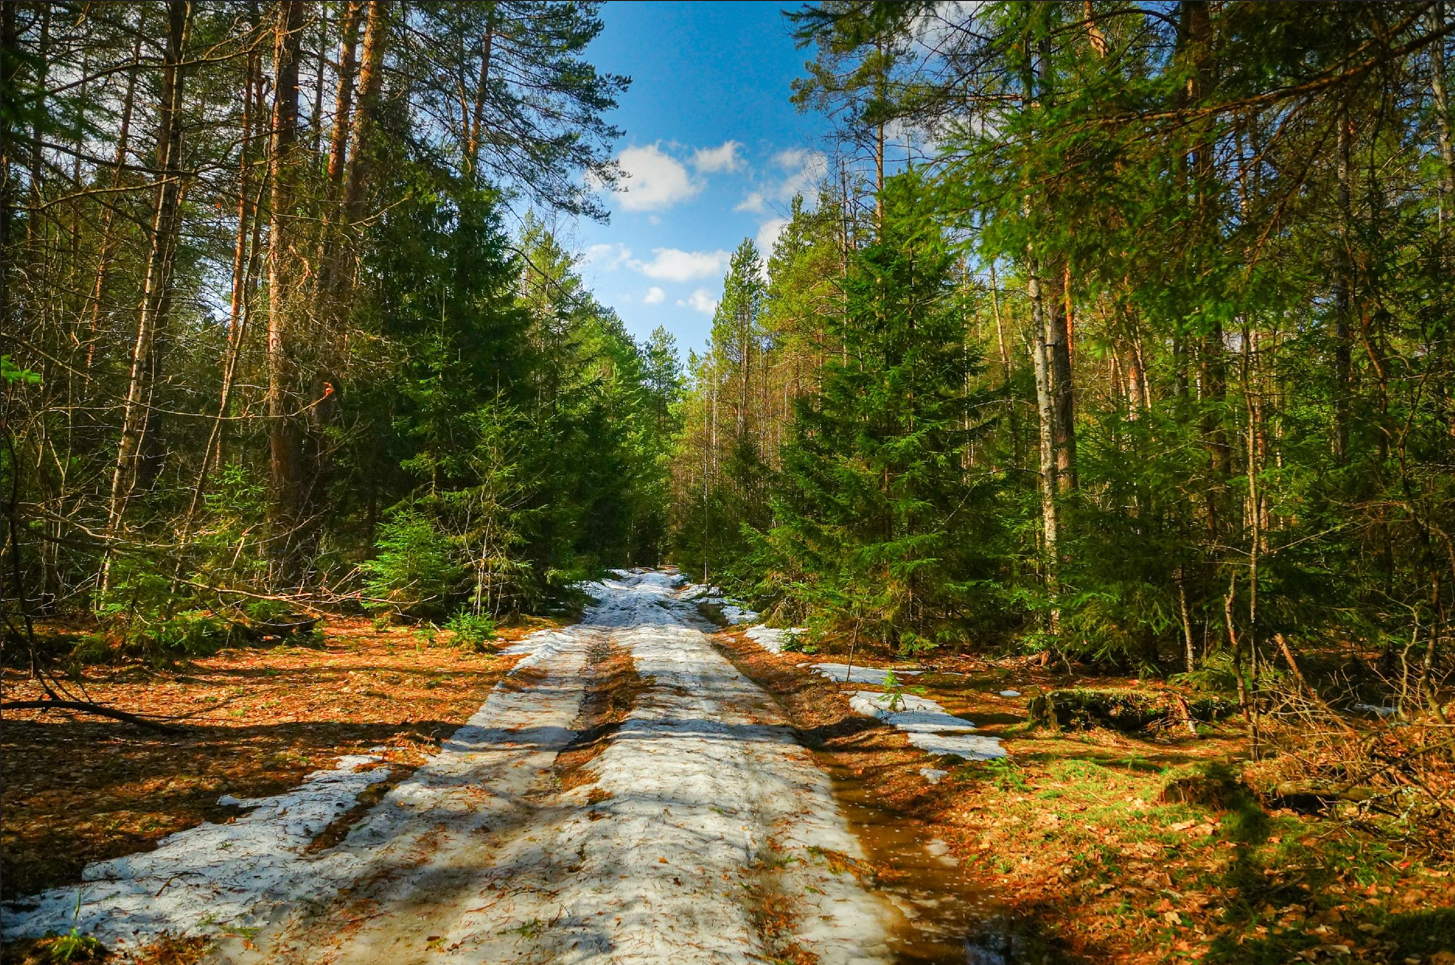
\includegraphics[width=170mm]{./img/march1.png}
	\caption{Исходное изображение для смешивания}
	\label{img:march}
\end{figure}

На рисунке \ref{img:result} изображен результат смешивания графа \ref{img:graph} и исходного изображения мартовского пейзажа \ref{img:march}.
\begin{figure}[ht!]
	\centering
	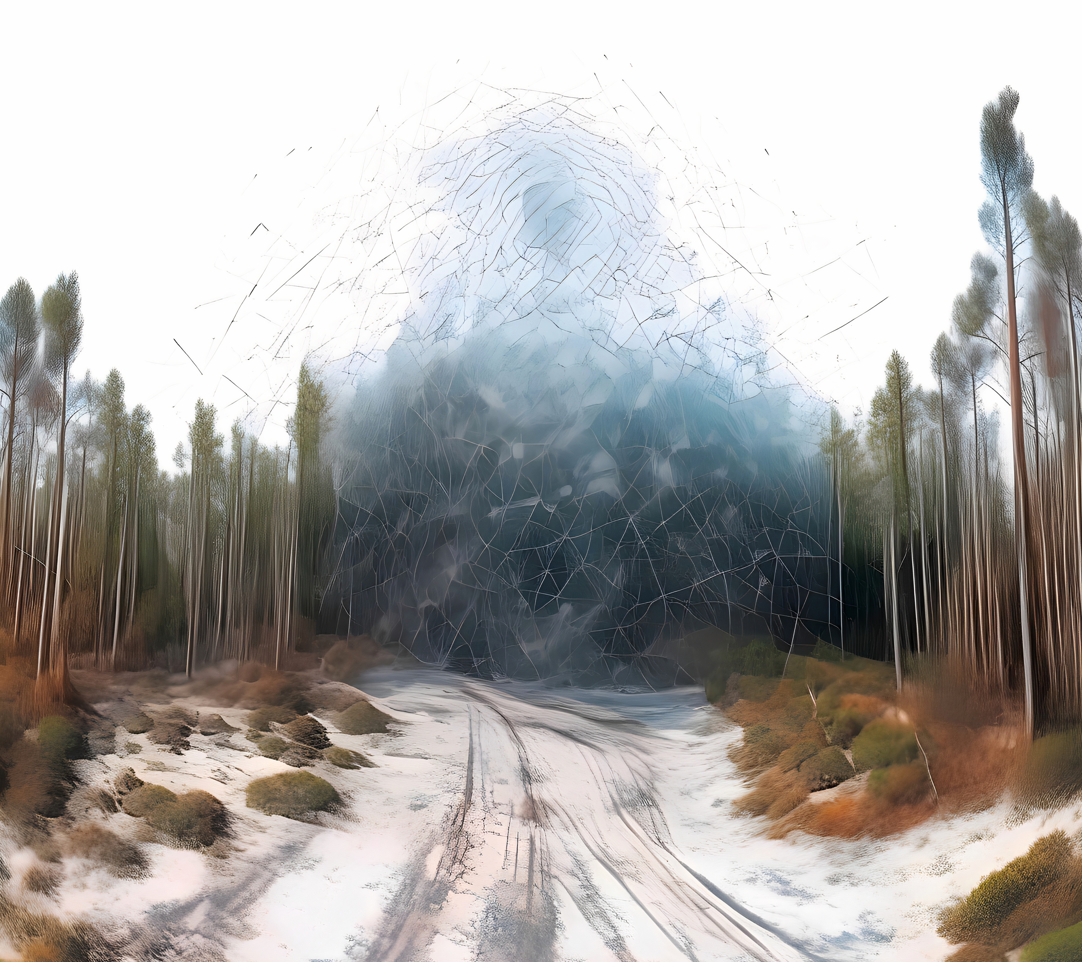
\includegraphics[width=170mm]{./img/result1.png}
	\caption{Результат смешивания изображений}
	\label{img:result}
\end{figure}